\section{Auswertung}


    \subsection{Widerstand}


    Das Außmessen der Proben ergibt:
    \begin{table}[H]
        \centering
        %\caption{Die Messwerte}
        \begin{tabular}{ S  S [table-format=1.5] S [table-format=1.4] S [table-format=1.6] S [table-format=1.6] S [table-format=1.2]}
            \toprule
            {Metall} & {Höhe}& {Breite}& {Dicke}& {Durchmesser} & {Länge}\\
            \midrule
            \text{Zink} & 0.02603  & 0.0280 & 0.000430 & 0.000263 & 1.73\\
            \text{Kupfer} & 0.04406  & 0.0253 & 0.000018 &  0.0001052 & 1.73\\
            \bottomrule
        \end{tabular}
    \caption{Eine Tabelle zu den Dimensionen der Metall Proben}
    \label{tab:Dimensionen}
    \end{table}
    \noindent Die Messwerte zur Höhe, Breite und Dicke beziehen sich hier auf die Metallplatte, die Messwerte zum Durchmesser und zur Länge
    beschreiben das jeweilige Kabel zur Berechnung des Widerstandes. Hier gehen wir jeweils von einer Ungenauigkeit von einem Prozent 
    des jeweiligen Messwertes aus.\\
    \noindent Der Widerstand eines Metalls berechnet sich Mittels 
    
    \begin{equation}
        U = R * I
    \end{equation}

    Die Berechnung des Widerstandes gibt eine Reihe an Widerstaenden \ref{tab:ErgWider}, der Mittelwert dieser Reihen ergibt dann einen Widerstand 
    fuer Zink und Kupfer:

    \begin{align}
        R_{\text{Zink}} &= \SI{13.68+-0.23}{\milli\ohm}\\
        R_{\text{Kupfer}} &= \SI{7.73+-0.05}{\milli\ohm}
    \end{align}

    Der spezifische Widerstand eines Metalls berechnet sich nun mittels der Formel

    \begin{equation}
        \rho = \frac{RA}{l}
    \end{equation}

    mit $R$ dem Widerstand, $A$ der Querschnittsflaeche und $l$ der Laenge des Kabels.
    Somit ergibt sich mit denn Werten aus \ref{tab:Dimensionen} und den berechneten Widerstaenden der spezifische Widerstand:

    \begin{align}
        \rho &= \SI{1.72+-0.05}{\nano\ohm\meter}\\
        \rho &= \SI{0.16+-03.1}{\nano\ohm\meter}
    \end{align}

    \subsection{Hall-Effekt}
    Zur Berechnung der Hall Spannung wird zunaechst das Magnetfeld der Spule in abhaengigkeit von der Stromstaerke bestimmt.

    \begin{figure}[H]
        \centering
        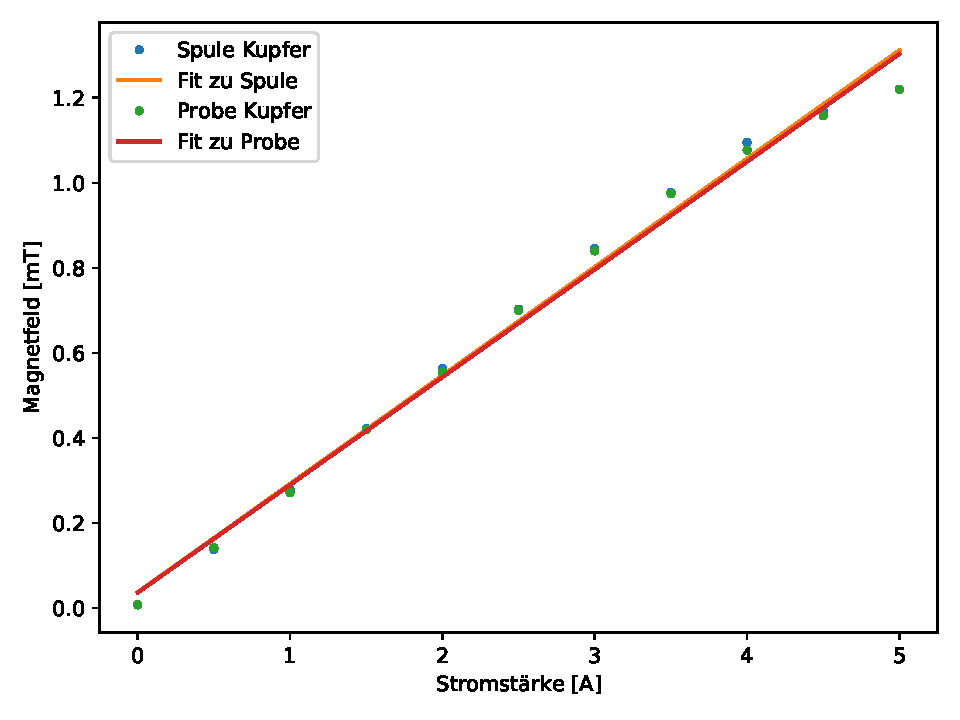
\includegraphics[width=0.7\textwidth]{build/Magnetfeld.pdf}
        \caption{Ein Plot der Magnetfeldstaerke gegen die Stromstaerke.}
        \label{img:Magnetfeld}
    \end{figure}

    In diesem Plot sind die Magnetfelder bei steigender und abfallender Stromstaerke \ref{tab:messMag} und der jeweilige lineare Fit zu den 
    Messwerten eingezeichnet.
    Die Ausgleichsgerade der Form $\text{a}\cdot x = \text{b}$ hat dann die Werte:
    \begin{align}
        \text{a} & = \num{254(5)e-3}\\
        \text{b} & = \num{36.750(16)e-3}
    \end{align}
    Und gibt nun in allen folgenden Rechnungen einen Wert für das Magnetfeld wenn nur ein Wert für den Spulenstrom bekannt ist.

    In den folgenden Plots ist sind die Messergebnisse der Hallspannung aufgetragen mit denen die weiteren Rechnungen ausgeführt werden.
    Die Zahlenwerte sind hier \ref{teb:messUH1},\ref{teb:messUH2},\ref{teb:messUH3},\ref{teb:messUH4} zu finden.

    \begin{figure}[H]
        \centering
        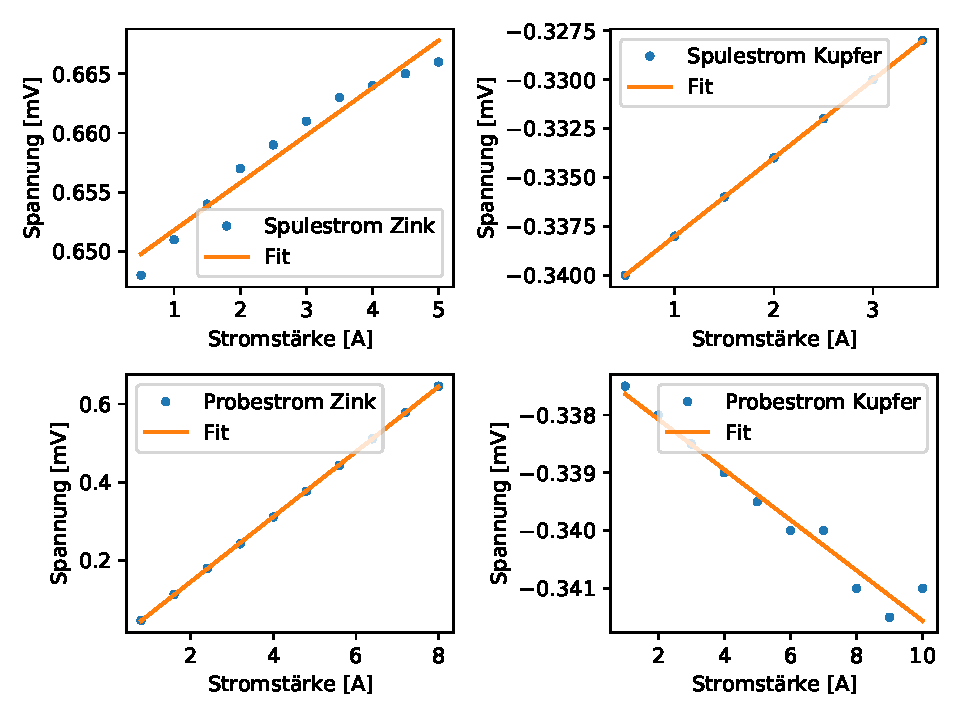
\includegraphics[width=1.1\textwidth]{build/Hall.pdf}
        \caption{Ein Plot der Hall Spannungen gegen die Stromstaerke.}
        \label{img:messHall}
    \end{figure}
    
     
    \subsection{Ladungsträger pro Volumen}
    

    Zur Berechnung der Hall Spannung wird zunaechst das Magnetfeld der Spule in abhaengigkeit von der Stromstaerke bestimmt.

    \begin{figure}[H]
        \centering
        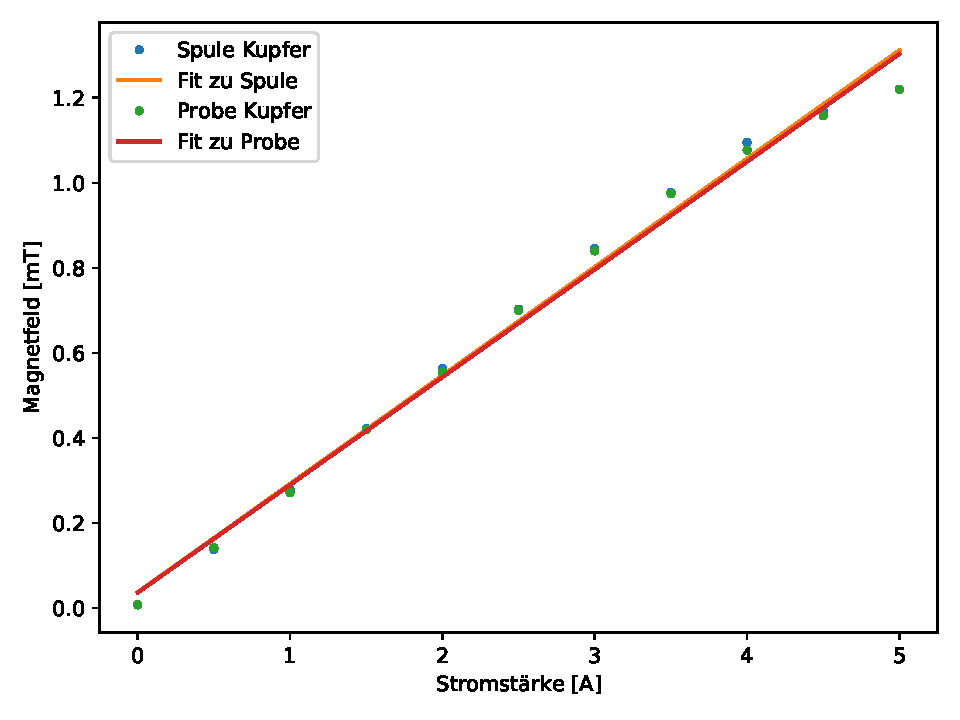
\includegraphics[width=0.7\textwidth]{build/Magnetfeld.pdf}
        \caption{Ein Plot der Magnetfeldstaerke gegen die Stromstaerke.}
        \label{img:Magnetfeld}
    \end{figure}

    In diesem Plot sind die Magnetfelder bei steigender und abfallender Stromstaerke \ref{tab:messMag} und der jeweilige lineare Fit zu den 
    Messwerten eingezeichnet.
    Die Ausgleichsgerade der Form $\text{a}\cdot x = \text{b}$ hat dann die Werte:
    \begin{align}
        \text{a} & = \num{254(5)e-3}\\
        \text{b} & = \num{36.750(16)e-3}
    \end{align}
    Und gibt nun in allen folgenden Rechnungen einen Wert für das Magnetfeld wenn nur ein Wert für den Spulenstrom bekannt ist


    Aus der Formel \ref{eqn:uhall} lässt sich nun eine Formel für die Ladungsträger pro Volumen herleiten:
    \begin{align}
        n &= \frac{-BI}{Ud\cdot\text{e}_0}
    \end{align}
    mit $B$ der magnetischen Feldstärke, $I$ der Stromstärke, $U$ der Hall-Spannung, $d$ der Dicke der jeweiligen Proben und $\text{e}_0$ der 
    elementar Ladung eines Elektron.

    Mit den angegeben Messwerten berechnen sich nun folgende Messwert:
    \begin{figure}[H]
        \centering
        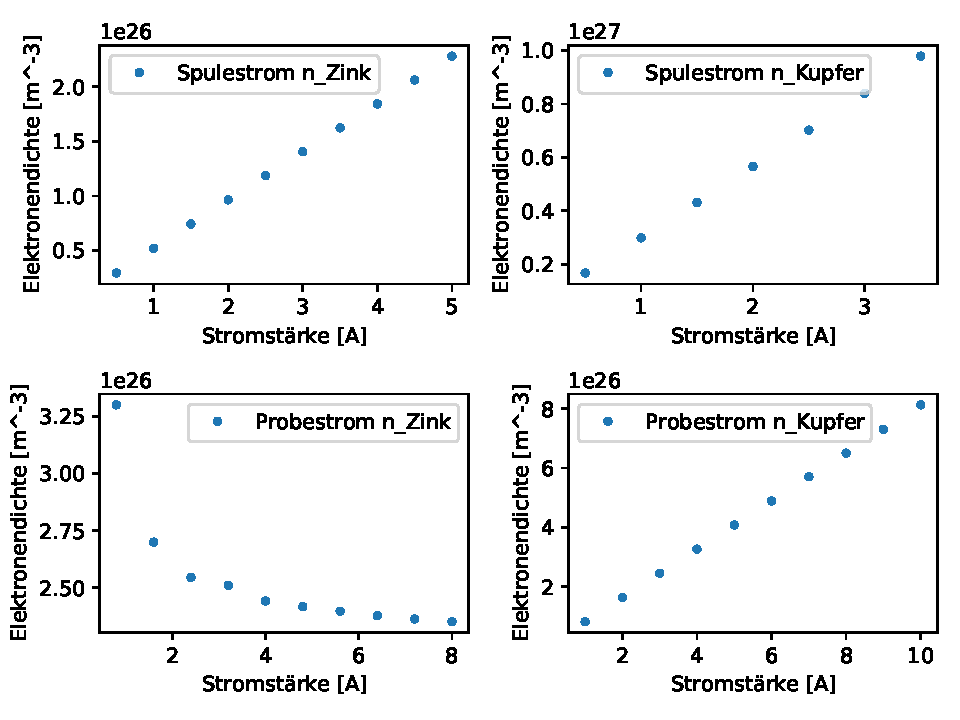
\includegraphics[width=1.1\textwidth]{build/n.pdf}
        \caption{Ein Plot der Elektronendichte gegen die Stromstaerke.}
        \label{img:elekdichte}
    \end{figure}
    Die durch die Plots veranschaulichten Werte sind auch in der Tabelle ?ref? zu finden.


    \subsection{Ladungsträger pro Atom}


    Die Anzahl der Atome pro Volumen berechnet sich mittels der Formel:
    \begin{equation}
        \frac{\text{Atome}}{\text{V}} = \frac{\rho \cdot \symup{N_A}}{\symup{m_{mol}}}
    \end{equation}
    Mit $\rho$ der Dichte des Metalls, $\symup{N_A}=\SI{6.02214076e23}{\per\mole}$ der Avogrado-Konstante und $\symup{m_mol}$ der 
    molaren Masse des Metalls.
    Aus dieser Formel ergibt sich direkt die Formel für Z die Anzahl der Ladungsträger pro Atom:
    \begin{equation}
        Z=\frac{n \cdot \symup{m_{mol}}}{\rho \cdot \symup{N_A}}
    \end{equation}
    Mit den stoffspezifischen Größen:
    \begin{table}[H]
        \centering
        %\caption{Die Messwerte}
        \begin{tabular}{ S  S [table-format=1.5] S [table-format=1.4] }
            \toprule
            {Metall} & {$\rho [\si{\gram\per\mole}]$}& {$\symup{m_{mol}}[\si{\gram\per\mole}]$}\\
            \midrule
            \text{Zink} &  7.14 & 65.38 \\
            \text{Kupfer} & 8.92 & 63.55 \\
            \bottomrule
        \end{tabular}
    \caption{Eine Tabelle mit stoffspezifischen Größen der Metalle}
    \label{tab:spez}
    \end{table}

    lässt sich nun Z berechnen. In den folgenden Plots ist Z für die unterschiedlichen Messreihen angegeben.
    \begin{figure}[H]
        \centering
        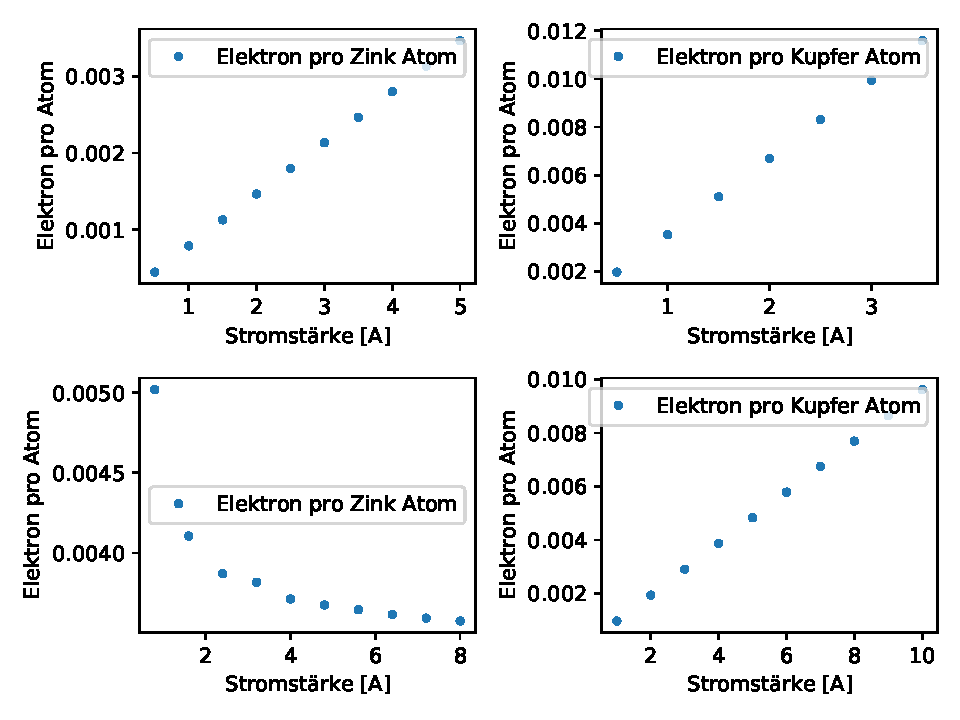
\includegraphics[width=1.1\textwidth]{build/Z.pdf}
        \caption{Ein Plot der Elektronendichte gegen die Stromstaerke.}
        \label{img:elekZahl}
    \end{figure}
    Die zugehörigen sind auch wieder in der Tabelle ?ref? zu finden.


    \subsection{mittlere Flugzeit}

    
    Die Formel \ref{eqn:rho} wir so umgestellt, dass wir folgende Formel erhalten:
    \begin{equation}
        \overline{\tau} =\frac{2}{n}\frac{\symup{m_0}}{\symup{e_0}^2 \cdot \rho}
    \end{equation}
    In dieser Formel rechnen wir wieder mit dem reziproken spezifischen Widerstand $\rho$ und der Elektronenmasse
    $\symup{m_0} = \SI{9.109e-31}{\kilogram}$. Das einsetzten der Werte für $n$ und $\rho$ ergibt dann folgende Werte ?ref?:

    \begin{figure}[H]
        \centering
        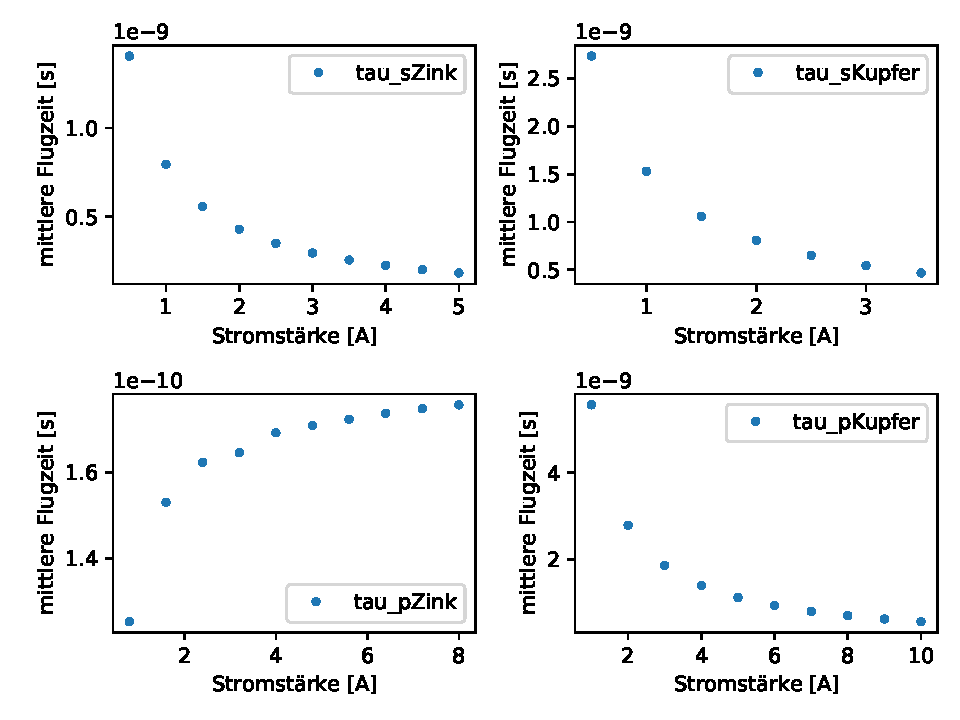
\includegraphics[width=1.1\textwidth]{build/tau.pdf}
        \caption{Ein Plot der mittleren Flugzeit gegen die Stromstaerke.}
        \label{img:tau}
    \end{figure}


    \subsection{mittlere Driftgeschwindigkeit}


    Die mittlere Driftgeschwindigkeit $\overline{v_d}$ berechnet sich aus:
    \begin{equation}
        \overline{v_d} = \frac{-n \cdot \symup{e_0}}{\symup{j}}
    \end{equation}
    mit der Stromdichte j = $\SI{1}{\ampere\per\milli\meter\squared}$.

    Einsetzten ergibt dann ?ref?:
    \begin{figure}[H]
        \centering
        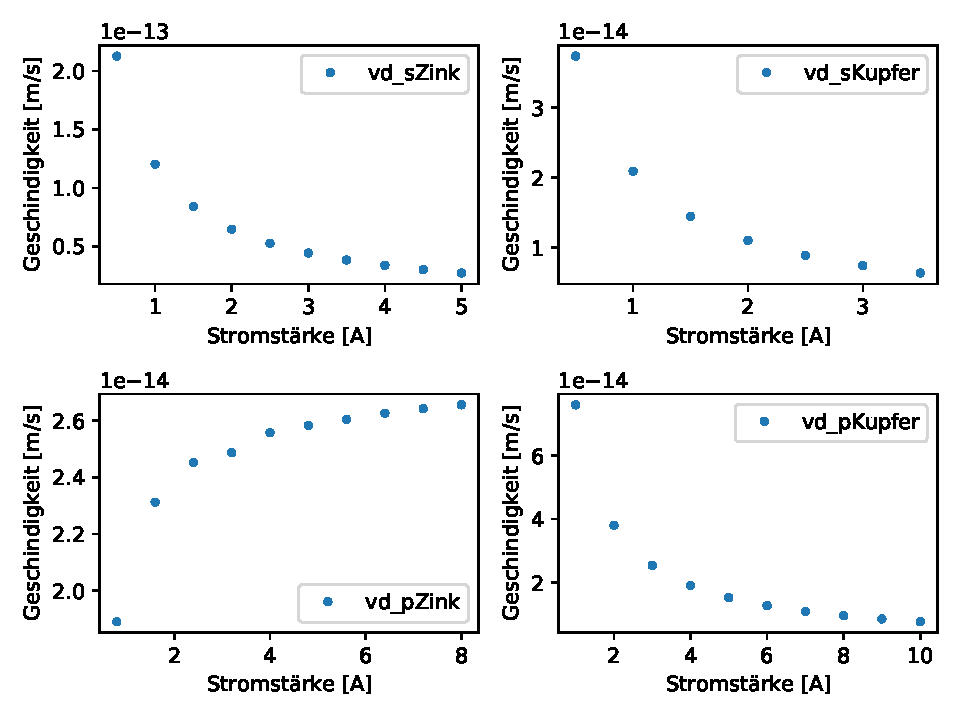
\includegraphics[width=1.1\textwidth]{build/Driftgeschwindigkeit.pdf}
        \caption{Ein Plot der Driftgeschwindigkeit gegen die Stromstaerke.}
        \label{img:vd}
    \end{figure}


    \subsection{Beweglichkeit}


    Die Formel
    \begin{equation}
        \mu= -\frac{1}{2}\frac{\symup{e_0}}{\symup{m_0}}\cdot   \overline{\tau}
    \end{equation}
    stellt eine Beziehung zwischen $\tau$ und $\mu$ auf, mit den Werten für $\tau$ ?ref? berechnen sich nun folgende Werte 
    für $\tau$ ?ref?:

    \begin{figure}[H]
        \centering
        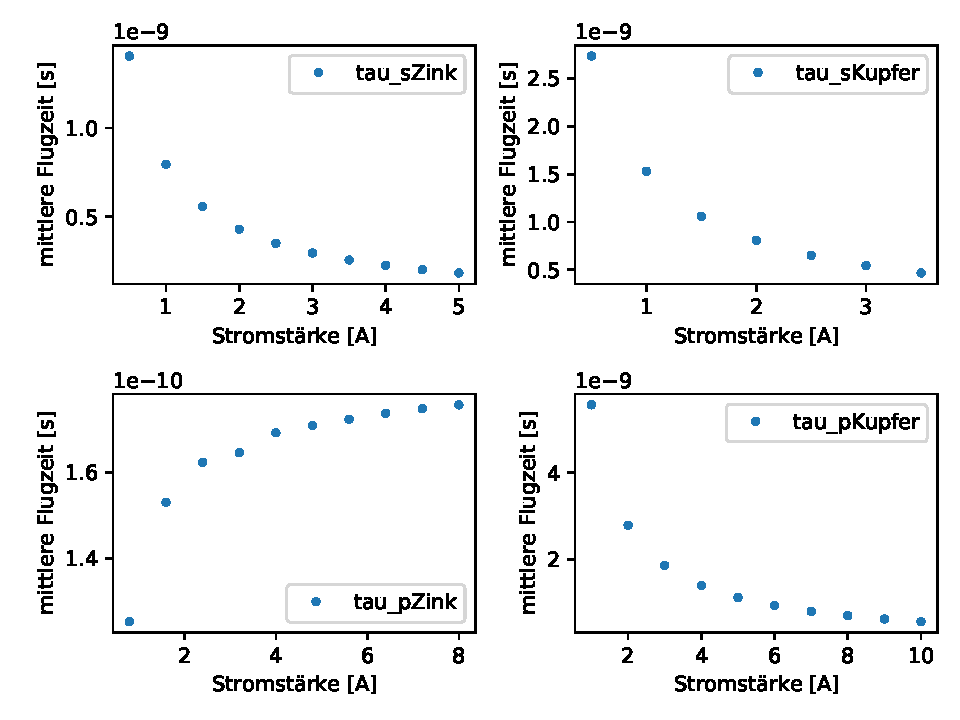
\includegraphics[width=1.1\textwidth]{build/tau.pdf}
        \caption{Ein Plot der Beweglichkeit gegen die Stromstaerke.}
        \label{img:Beweg}
    \end{figure}


    \subsection{Totalgeschwindigkeit}


    Für die Totalgeschwindigkeit wird zunaechst ein Wert für die Fermi-Energie berechnet werden, diese berechnet sich mittels der Formel:
    \begin{equation}
        E_F = \frac{\symup{h}^2}{2 \cdot \symup{m_0}}\sqrt{\left(\frac{3}{8\pi}\right)^2}
    \end{equation}
    Hier ist h das planksche Wirkungsquantum($\SI{6.626e-34}{\joule\second}$).
    Die Fermi-Energie berechnet sich zu: ?ref?

    \begin{figure}[H]
        \centering
        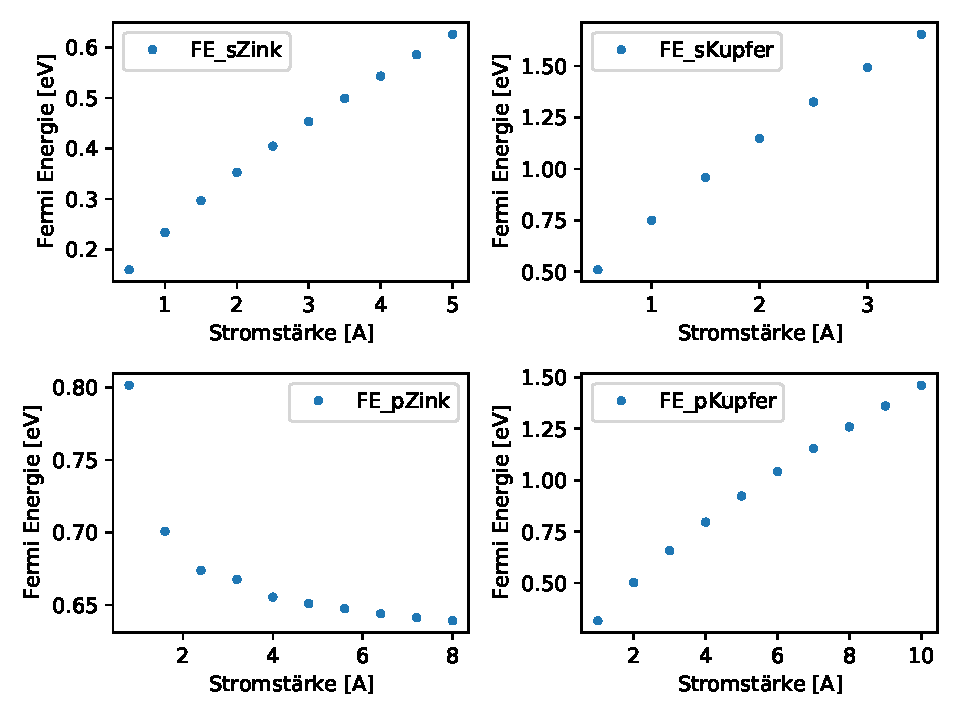
\includegraphics[width=1.1\textwidth]{build/Fermi.pdf}
        \caption{Ein Plot der Fermi-Energie gegen die Stromstaerke.}
        \label{img:FE}
    \end{figure}

    Mittels der Fermi-Energie lässt sich nun über 

    \begin{equation}
        |\overline{v}| \approx \sqrt{\frac{2E_F}{\symup{m_0}}} \nonumber
    \end{equation}

    die Totalgeschwindigkeit bestimmen: ?ref?

    \begin{figure}[H]
        \centering
        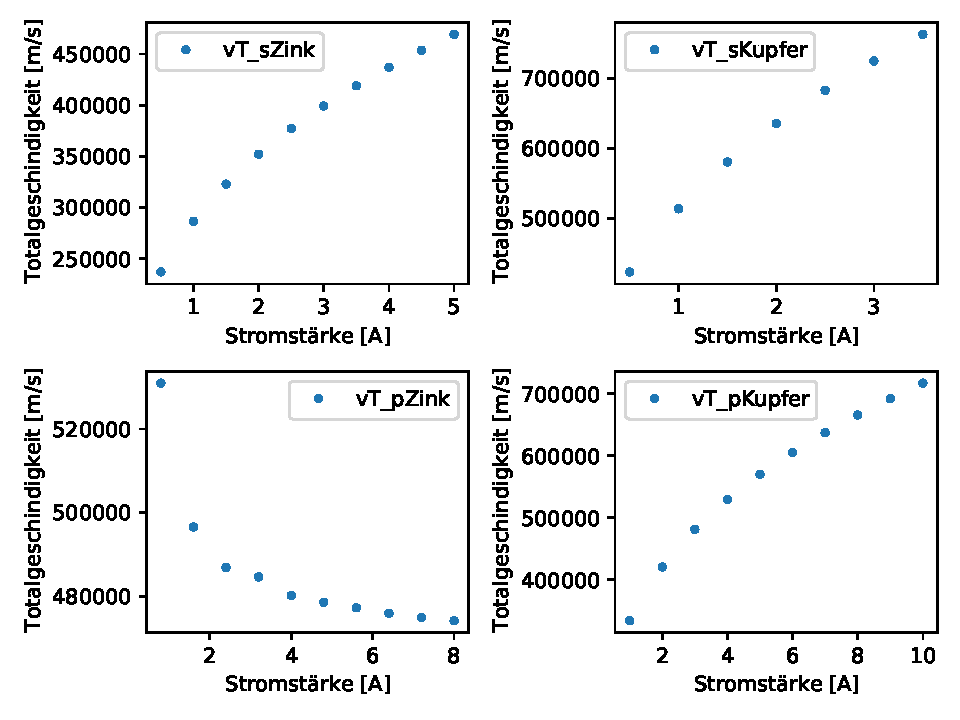
\includegraphics[width=1.1\textwidth]{build/Totalgeschwindigkeit.pdf}
        \caption{Ein Plot der Totalgeschwindigkeit gegen die Stromstaerke.}
        \label{img:vT}
    \end{figure}


    \subsection{mittlere freie Weglänge}


    Die mittlere freie Weglänge lässt sich nun mit der Totalgeschwindigkeit$|\overline{v}|$ und mittleren Flugzeit$\tau$ berechnen:
    \begin{equation}
        \overline{l} \approx \overline{\tau} \cdot |\overline{v}| \nonumber
    \end{equation}

    
    \begin{figure}[H]
        \centering
        \includegraphics[width=1.1\textwidth]{build/mittlere_Weglänge.pdf}
        \caption{Ein Plot der mittleren freien Weglänge gegen die Stromstaerke.}
        \label{img:mfl}
    \end{figure}
    Die Zahlenwerte zu den Plots befinden sich hier ?ref?

    \subsection{Elektronenleitung}
    Da von der Tatsache ausgegangen wird, dass Kupfer ein Elektronenleiter ist und bei Kupfer und Zink unterschiedliche Vorzeichen für
    die Hall-Spannung gemessen wurde, ist relativ Sicher, dass bei Zink die Löcherleitung überwiegt.





















    \section{Tabellen}

    \begin{table}[H]
        \centering
        %\caption{Die Messwerte}
        \begin{tabular}{ S [table-format=1.1] S [table-format=1.4] S [table-format=1.4]}
            \toprule
            {$\text{Stromstaerke}\si{\ampere}$} & {$\text{Spannung Zink}\si{\volt}$} & {$\text{Spannung Kupfer}\si{\volt}$}\\
            \midrule
            1.0          & 0.0141       & 0.0078\\     
            2.0          & 0.0277       & 0.0155\\     
            3.0          & 0.0411       & 0.0233\\      
            4.0          & 0.0555       & 0.0309\\      
            5.0          & 0.0683       & 0.0386\\      
            6.0          & 0.0815       & 0.0463\\      
            7.0          & 0.0947       & 0.0539\\
            8.0          & 0.1071       & 0.0615\\      
            9.0          & 0.1203       & 0.0688\\      
            10.0         & 0.1337       & 0.0765\\
            \bottomrule
        \end{tabular}
    \caption{Messwerte zur Berechnung der Widerstaende}
    \label{tab:messWider}
    \end{table}


    \begin{table}[H]
        \centering
        %\caption{Die Messwerte}
        \begin{tabular}{ S [table-format=1.1] S [table-format=1.4] }
            \toprule
            {$R_{\text{Kupfer}}\si{\ohm}$} & {$R_{\text{Zink}}\si{\ohm}$}\\
            \midrule
            0.01413 & 0.00783\\
            0.01385 & 0.00777\\
            0.01370 & 0.00777\\
            0.01387 & 0.00773\\
            0.01366 & 0.00772\\
            0.01358 & 0.00772\\
            0.01352 & 0.00770\\
            0.01338 & 0.00769\\
            0.01337 & 0.00764\\
            \bottomrule
        \end{tabular}
    \caption{Messwerte zur Berechnung der Widerstaende}
    \label{tab:ErgWider}
    \end{table}

    \begin{table}[H]
        \centering
        %\caption{Die Messwerte}
        \begin{tabular}{ S [table-format=1.1] S [table-format=1.3] S [table-format=1.1] S [table-format=1.3]}
            \toprule
            {$\text{Stromstaerke+}\si{\ampere}$} & {$\text{Magnetfeld+}\si{\tesla}$} & {$\text{Stromstaerke-}\si{\ampere}$}& {$\text{Magnetfeld-}\si{\tesla}$}\\
            \midrule
            0.5          & 0.142    & 5.0          & 1.220 \\
            1.0          & 0.272    & 4.5          & 1.169 \\
            1.5          & 0.420    & 4.0          & 1.095 \\
            2.0          & 0.556    & 3.5          & 0.977 \\
            2.5          & 0.700    & 3.0          & 0.845 \\
            3.0          & 0.840    & 2.5          & 0.703 \\
            3.5          & 0.975    & 2.0          & 0.563 \\
            4.0          & 1.077    & 1.5          & 0.422 \\
            4.5          & 1.158    & 1.0          & 0.279 \\
            5.0          & 1.220    & 0.5          & 0.138 \\
            \bottomrule
        \end{tabular}
    \caption{Messwerte zur Berechnung der Widerstaende}
    \label{tab:messMag}
    \end{table}

    \begin{table}[H]
        \centering
        %\caption{Die Messwerte}
        \begin{tabular}{ S [table-format=1.1] S [table-format=1.3] }
            \toprule
            {$\text{Stromstaerke+}\si{\ampere}$} & {$\text{Magnetfeld+}\si{\tesla}$}\\
            \midrule
            0.5                   & 1.220 \\
            1.0                   & 1.169 \\
            1.5                   & 1.095 \\
            2.0                   & 0.977 \\
            2.5                   & 0.845 \\
            3.0                   & 0.703 \\
            3.5                   & 0.563 \\
            4.0                   & 0.422 \\
            4.5                   & 0.279 \\
            5.0                   & 0.138 \\
            \bottomrule
        \end{tabular}
    \caption{Messwerte zur Berechnung der Widerstaende}
    \label{tab:messMag}
    \end{table}
  

    \begin{table}[H]
        \centering
        %\caption{Die Messwerte}
        \begin{tabular}{S [table-format=1.1] S [table-format=1.3] S [table-format=1.3] }
            \toprule
            {$\text{Stromstärke}\si{\ampere}$} & {$\text{Hallspannung steigend }\si{\milli\volt}$} & {$\text{Hallspannung fallend }\si{\milli\volt}$}\\
            \midrule
            0.5   & 0.648 & 0.648\\
            1.0   & 0.651 & 0.651\\
            1.5   & 0.654 & 0.654\\
            2.0   & 0.657 & 0.657\\
            2.5   & 0.659 & 0.659\\
            3.0   & 0.661 & 0.661\\
            3.5   & 0.663 & 0.663\\
            4.0   & 0.664 & 0.664\\
            4.5   & 0.665 & 0.665\\
            5.0   & 0.666 & 0.666\\
            \bottomrule
        \end{tabular}
    \caption{Messwerte der Hallspannung von Zink bei konstantem Probenstrom}
    \label{tab:messMag}
    \end{table}

    \begin{table}[H]
        \centering
        %\caption{Die Messwerte}
        \begin{tabular}{S [table-format=1.1] S [table-format=1.3] S [table-format=1.3] }
            \toprule
            {$\text{Stromstärke}\si{\ampere}$} & {$\text{Hallspannung steigend }\si{\milli\volt}$} & {$\text{Hallspannung fallend }\si{\milli\volt}$}\\
            \midrule
            0.5   & -0.340 & -0.340\\
            1.0   & -0.338 & -0.338\\
            1.5   & -0.336 & -0.336\\
            2.0   & -0.334 & -0.334\\
            2.5   & -0.332 & -0.332\\
            3.0   & -0.330 & -0.330\\
            3.5   & -0.328 & -0.328\\
            \bottomrule
        \end{tabular}
    \caption{Messwerte der Hallspannung von Zink bei konstantem Probenstrom}
    \label{tab:messUH1}
    \end{table}

    \begin{table}[H]
        \centering
        %\caption{Die Messwerte}
        \begin{tabular}{S [table-format=1.1] S [table-format=1.3] S [table-format=1.3] }
            \toprule
            {$\text{Stromstärke}\si{\ampere}$} & {$\text{Hallspannung steigend }\si{\milli\volt}$} & {$\text{Hallspannung fallend }\si{\milli\volt}$}\\
            \midrule
            0.5   & -0.340 & -0.340\\
            1.0   & -0.338 & -0.338\\
            1.5   & -0.336 & -0.336\\
            2.0   & -0.334 & -0.334\\
            2.5   & -0.332 & -0.332\\
            3.0   & -0.330 & -0.330\\
            3.5   & -0.328 & -0.328\\
            \bottomrule
        \end{tabular}
    \caption{Messwerte der Hallspannung von Kupfer bei konstantem Probenstrom}
    \label{tab:messUH2}
    \end{table}


    \begin{table}[H]
        \centering
        %\caption{Die Messwerte}
        \begin{tabular}{S [table-format=1.1] S [table-format=1.3] S [table-format=1.3] }
            \toprule
            {$\text{Stromstärke}\si{\ampere}$} & {$\text{Hallspannung steigend }\si{\milli\volt}$} & {$\text{Hallspannung fallend }\si{\milli\volt}$}\\
            \midrule
            0.8 & 0.045 & 0.047\\
            1.6 & 0.109 & 0.116\\
            2.4 & 0.174 & 0.184\\
            3.2 & 0.234 & 0.250\\
            4.0 & 0.304 & 0.318\\
            4.8 & 0.365 & 0.389\\
            5.6 & 0.431 & 0.456\\
            6.4 & 0.495 & 0.527\\
            7.2 & 0.560 & 0.597\\
            8.0 & 0.626 & 0.666\\
            \bottomrule
        \end{tabular}
    \caption{Messwerte der Hallspannung von Zink bei konstantem Spulenstrom}
    \label{tab:messUH3}
    \end{table}
    

    \begin{table}[H]
        \centering
        %\caption{Die Messwerte}
        \begin{tabular}{S [table-format=1.1] S [table-format=1.3] S [table-format=1.3] }
            \toprule
            {$\text{Stromstärke}\si{\ampere}$} & {$\text{Hallspannung steigend }\si{\milli\volt}$} & {$\text{Hallspannung fallend }\si{\milli\volt}$}\\
            \midrule
            1.00 & -0.338 & -0.337  \\
            2.00 & -0.340 & -0.336  \\
            3.00 & -0.342 & -0.335  \\
            4.00 & -0.343 & -0.335  \\
            5.00 & -0.345 & -0.334  \\
            6.00 & -0.347 & -0.333  \\
            7.00 & -0.348 & -0.332  \\
            8.00 & -0.350 & -0.332  \\
            9.00 & -0.351 & -0.332  \\
            10.00& -0.352 & -0.330  \\
            \bottomrule
        \end{tabular}
    \caption{Messwerte der Hallspannung von Kupfer bei konstantem Spulenstrom}
    \label{tab:messUH4}
    \end{table}